\documentclass[]{article}

\usepackage[left=2.00cm, right=2.00cm, top=2.00cm, bottom=2.00cm]{geometry}
\usepackage[spanish,es-noshorthands]{babel}
\usepackage[utf8]{inputenc} % para tildes y ñ
\usepackage{graphicx} % para las figuras
\usepackage{xcolor}
\usepackage{listings} % para el código fuente en c++

\lstdefinestyle{customc}{
  belowcaptionskip=1\baselineskip,
  breaklines=true,
  frame=single,
  xleftmargin=\parindent,
  language=C++,
  showstringspaces=false,
  basicstyle=\footnotesize\ttfamily,
  keywordstyle=\bfseries\color{green!40!black},
  commentstyle=\itshape\color{gray!40!gray},
  identifierstyle=\color{black},
  stringstyle=\color{orange},
}
\lstset{style=customc}


%opening
\title{Práctica 3. Divide y vencerás}
\author{Santos Romero Alvaro \\ % mantenga las dos barras al final de la línea y este comentario
alvarosantosrom9@gmail.com \\ % mantenga las dos barras al final de la línea y este comentario
Teléfono: xxxxxxxx \\ % mantenga las dos barras al final de la linea y este comentario
NIF: xxxxxxxxm \\ % mantenga las dos barras al final de la línea y este comentario
}


\begin{document}

\maketitle

%\begin{abstract}
%\end{abstract}

% Ejemplo de ecuación a trozos
%
%$f(i,j)=\left\{ 
%  \begin{array}{lcr}
%      i + j & si & i < j \\ % caso 1
%      i + 7 & si & i = 1 \\ % caso 2
%      2 & si & i \geq j     % caso 3
%  \end{array}
%\right.$

\begin{enumerate}
\item Describa las estructuras de datos utilizados en cada caso para la representación del terreno de batalla. 

Escriba aquí su respuesta al ejercicio 1. 

% Elimine los símbolos de tanto por ciento para descomentar las siguientes instrucciones e incluir una imagen en su respuesta. La mejor ubicación de la imagen será determinada por el compilador de Latex. No tiene por qué situarse a continuación en el fichero en formato pdf resultante.
%\begin{figure}
%\centering
%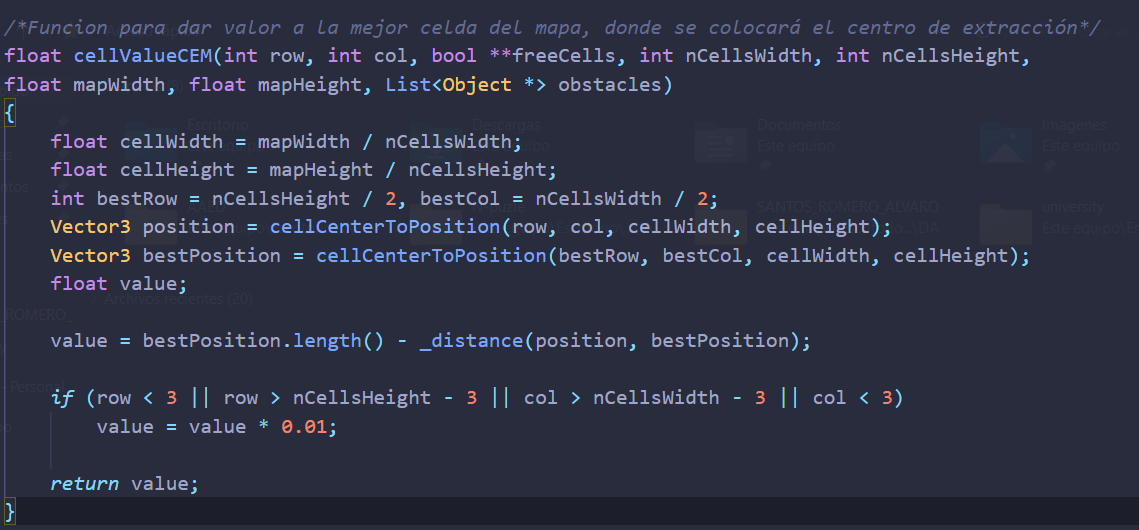
\includegraphics[width=0.7\linewidth]{./defenseValueCellsHead} % no es necesario especificar la extensión del archivo que contiene la imagen
%\caption{Estrategia devoradora para la mina}
%\label{fig:defenseValueCellsHead}
%\end{figure}

\item Implemente su propia versión del algoritmo de ordenación por fusión. Muestre a continuación el código fuente relevante. 

Escriba aquí su respuesta al ejercicio 2.


\item Implemente su propia versión del algoritmo de ordenación rápida. Muestre a continuación el código fuente relevante. 

ALGORITMO DE ORDENACION RAPIDA O QUICKSORT.


Especificación del algoritmo:

-Algoritmo Divide y Vencerás perteneciente al esquema de Partición.

-Recibe un (std::vector<t> &array, int low, int high), donde low y high representa el rango desde 0 hasta tam -1.  
-Precondiciones: Vector t esté inicializado
-Postcondiciones: Devuelve la lista de t elementos ordenados.

Al igual que la versión vista en teoría, el algoritmo utiliza un parámetro p (pivote) para reorganizar el
vector a partir del cual a la derecha de este estarán los elementos mayores y a la izquierda los menores.

template <class t>
void quickSort(std::vector<t>& array, int low, int high) {
  if (low < high) {
      
    int pi = partition(array, low, high);

    quickSort(array, low, pi - 1);

    quickSort(array, pi + 1, high);
  }
}

template <class t>
int partition(std::vector<t>& array, int low, int high) {
    
  t pivot = array[high];
  
  int i = (low - 1);

  for (int j = low; j < high; j++) {
    if (array[j] <= pivot) {
      i++;  
      std::swap(array[i], array[j]);
    }
  }
  
  std::swap(array[i + 1], array[high]);
  
  return (i + 1);
}


\item Realice pruebas de caja negra para asegurar el correcto funcionamiento de los algoritmos de ordenación implementados en los ejercicios anteriores. Detalle a continuación el código relevante.

Escriba aquí su respuesta al ejercicio 4.

\item Analice de forma teórica la complejidad de las diferentes versiones del algoritmo de colocación de defensas en función de la estructura de representación del terreno de batalla elegida. Comente a continuación los resultados. Suponga un terreno de batalla cuadrado en todos los casos. 

Escriba aquí su respuesta al ejercicio 5.

\item Incluya a continuación una gráfica con los resultados obtenidos. Utilice un esquema indirecto de medida (considere un error absoluto de valor 0.01 y un error relativo de valor 0.001). Considere en su análisis los planetas con códigos 1500, 2500, 3500,..., 10500. Incluya en el análisis los planetas que considere oportunos para mostrar información relevante.

\begin{lstlisting}
// sustituya este codigo por su respuesta
void placeDefenses(...) {

    List<Defense*>::iterator currentDefense = defenses.begin();
    while(currentDefense != defenses.end() && maxAttemps > 0) {

        (*currentDefense)->position.x = ((int)(_RAND2(nCellsWidth))) * cellWidth + cellWidth * 0.5f;
        ...
        ++currentDefense;
    }
}
\end{lstlisting}

\end{enumerate}

Todo el material incluido en esta memoria y en los ficheros asociados es de mi autoría o ha sido facilitado por los profesores de la asignatura. Haciendo entrega de este documento confirmo que he leído la normativa de la asignatura, incluido el punto que respecta al uso de material no original.

\end{document}
